\documentclass[a4paper,10pt]{article}
\usepackage[utf8]{inputenc}
\usepackage[T1]{fontenc}
\usepackage{lmodern}	
\usepackage[italian]{babel}

\usepackage{amsmath}
\usepackage{amsfonts}
\usepackage{amssymb}

\usepackage{graphicx}
\usepackage[dvipsnames]{xcolor}  %colori

\usepackage[left=2cm,right=2cm,top=2cm,bottom=2cm]{geometry}
\geometry{a4paper}

\usepackage{verbatim}
\usepackage{lipsum}

\usepackage{booktabs}
\usepackage{subfig}
\usepackage{float}
\usepackage{wrapfig}

\usepackage[colorlinks=true, linkcolor=black, urlcolor=blue, citecolor=darkgray, filecolor=darkgray]{hyperref}   %per gli hyperlink
\usepackage[italian, sort, noabbrev, capitalise]{cleveref}
\usepackage[bottom]{footmisc}

\usepackage[cdot, thickqspace, squaren]{SIunits}
% macro
\def\code#1{\texttt{#1}}

\title{Esercitazione 14: Misura della costante di assorbimento del mylar\\ usando un
	amplificatore lock-in}
\author{Gruppo BL \\ Candido Alessandro, Luzio Andrea, Mazziotti Fabrizio}

\begin{document}

\maketitle

\section{Scopo e Strumentazione}
In questa esercitazione si vuole effettuare una misura di assorbimento della luce di uno spessore di mylar facendo uso di un amplificatore sincrono sensibile alla fase, o lock-in.
\newline

\noindent La strumentazione è quella solitamente presente sul banco di lavoro, e inoltre si è usato:
\begin{itemize}
	\item TL082: JFET input dual op-amp (x1);
	\item TL081: JFET input op-amp (x4);
	\item SN7400: quad NAND gates;
	\item DG441: quad CMOS analog switch;
	\item 2N1711, BC182: NPN transistors;
	\item LED rosso; fotodiodo.
\end{itemize}

\subsubsection*{Schema complessivo}

Lo schema a blocchi del circuito è riportato in \cref{fig:blocks}.

\begin{figure}[H]
	\centering
	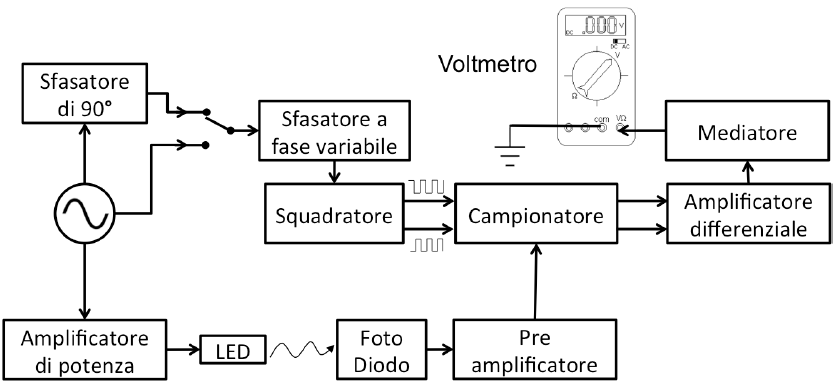
\includegraphics[width=\textwidth]{../grafici/Blocks.png}
	\vspace*{10pt}
	\caption{Schema a blocchi del circuito complessivo.}
	\label{fig:blocks}
\end{figure}

\pagebreak

\section{Implementazione dei blocchi di circuito}

\subsection{Amplificatore di potenza}

\begin{wrapfigure}{L}{0.5\textwidth}
	\vspace{-10pt}
	\centering
	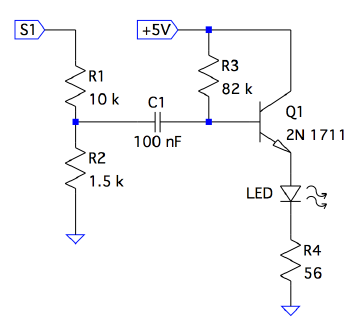
\includegraphics[width=0.5\textwidth]{../grafici/PowerAmp.png}
	\vspace{-12pt}
	\caption{Schema del circuito: amplificatore di potenza.}
	\label{fig:powamp}
	\vspace{-12pt}
\end{wrapfigure}

L'amplificatore di potenza, il cui circuito è mostrato in \cref{fig:powamp}, consiste a sua volta di due parti molto semplici:

\begin{itemize}
	\item un partitore di tensione, formato dalle resistenze $ R_1 $ e $ R_2 $;
	\item il circuito polarizzatore del transistor $ Q_1 $.
\end{itemize}

Il primo è un semplice partitore che riduce di quasi un fattore $ 10 $ la tensione in arrivo da $ S_1 $.
Nel secondo il ruolo di circuito polarizzatore è svolto interamente dalla parte superiore in \cref{fig:powamp}, cioè dalla resistenza $ R_3 $ e le connessioni a $ + \unit{5}{V} $ (e ovviamente dal collegamento a terra all'emettitore), mentre la resistenza $ R_4 $ serve principalmente a proteggere il LED.

Il condensatore interposto fra i due sottocircuiti ha lo scopo di evitare che le componenti in continua della polarizzazione del transistor fluiscano nell'altro, e allo stesso tempo lascia passare i segnali oscillanti in input.

Il transistor, montato in configurazione ad emettitore comune, viene qui usato come amplificatore di potenza per alimentare il LED.
\newline

Una volta montato questo sottocircuito si è verificato che il LED fosse acceso, come indicato.
Si riporta il segnale in tensione acquisito in \cref{fig:LED}.

\begin{figure}[H]
	\centering
	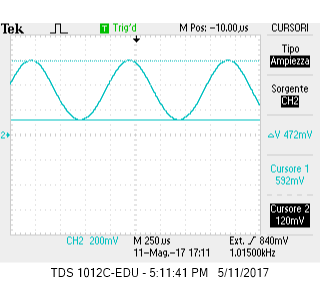
\includegraphics[width=0.5\textwidth]{../grafici/ledr4.png}
	\caption{Acquisizione del segnale all'uscita del LED.}
	\label{fig:LED}
\end{figure}

% Scrivere da qualche parte cosa si manda in ingresso!: In S1 collegare un segnale sinusoidale di frequenza 1 kHz ed ampiezza 6 VPP prelevato dal generatore di funzioni. Comunque ho messo la foto e lo ho scritto nella parte dello sfasatore, eventualmente si deve poi togliere da li


\subsection{Preamplificatore}

\begin{wrapfigure}{R}{0.5\textwidth}
	\vspace{-10pt}
	\centering
	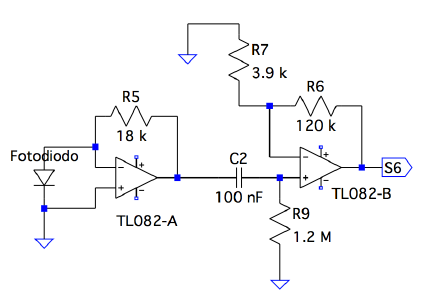
\includegraphics[width=0.5\textwidth]{../grafici/PreAmp.png}
	\vspace{-12pt}
	\caption{Schema del circuito: preamplificatore.}
	\label{fig:preamp}
	\vspace{-12pt}
\end{wrapfigure}

Il preamplificatore è anch'esso costituito di tre parti:
\begin{itemize}
	\item un primo operazionale ha lo scopo di amplificare la piccola differenza di potenziale che si genera ai capi del fotodiodo;
	\item un filtro passa-alto elimina tutte le componenti del segnale con frequenza superiore a quella con cui è alimentato il diodo;
	\item un secondo operaionale, montato in configurazione di amplificatore non invertente.
\end{itemize}

Il primo operazionale è montato nella configurazione di amplificatore invertente: a causa del feedback negativo si può applicare il metodo del cortocircuito virtuale, e porre $ v_- \simeq v_+ = 0 $.
La corrente che scorre dentro il fotodiodo sarà la stessa che scorre nella resistenza $ R_5 $, a causa dell'altissima impedenza di ingresso dell'OpAmp, per cui il valore dell'uscita è determinato da questa corrente e il valore della resistenza $ R_5 $.
In questo modo per mezzo dell'OpAmp il fotodiodo non è direttamente caricato con gli step successivi del circuito, i quali preleveranno corrente dall'operazionale, e non direttamente dal fotodiodo.

Il filtro è dimensionato in modo tale da avere una frequenza di taglio prossima a $ \unit{1}{\kilo\hertz} $, data dai valori dei componenti $ C_2 $ e $ R_9 $.

Il secondo OpAmp, come si è detto, costituisce assieme alle resistenze $ R_6 $ e $ R_7 $ un amplificatore non invertente, la cui amplificazione è data dal rapporto $ R_6/R_7 $ (più esattamente è $ 1 + R_6/R_7 $).
\newline

Si è osservato il segnale sull'uscita $ S_6 $ (riportato in \cref{fig:s6}) e si è misurata per esso un'ampiezza pari a $ \unit{3.54 \pm 0.11}{\volt} $.

\begin{figure}[H]
	\centering
	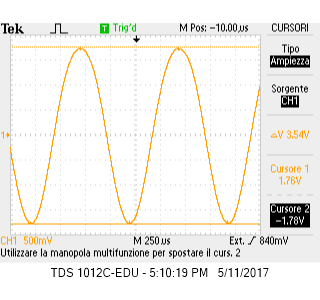
\includegraphics[width=0.5\textwidth]{../grafici/s6.png}
	\vspace{-10pt}
	\caption{Segnale sull'uscita $ S_6 $.}
	\label{fig:s6}
\end{figure}

\subsubsection*{Misure e rumore}

Si è misurata l'uscita $ S_6 $ ponendo alcune piastrine, e si riporta in \cref{tab:s6} i risultati ottenuti.

\begin{table}[H]
	\centering
	\begin{tabular}{cc}
		$ S_6 (V)$ & $ N^\circ sheets $\\
		\hline
		$ 2.76 \pm 0.09$	& 1\\
		$ 2.26 \pm 0.07$	& 2\\
		$ 1.84 \pm 0.06$	& 3\\
		$ 1.48 \pm 0.05$	& 4\\
		$ 1.22 \pm 0.04$	& 5\\
		$ 1.02 \pm 0.03$	& 6\\		
	\end{tabular}
\caption{Misure della tensione sull'uscita $ S_6 $ in funzione del numero di piastrine.}
\label{tab:s6}
\end{table}

Si è inoltre valutato qualitativamente l'effetto del rumore: la componente prevalente di esso era dovuta alla luce ambientale, tolta questa il rumore residuo era confrontabile con l'errore dell'oscilloscopio.
Per eliminare l'effetto della luce ambientale (la quale produceva oscillazioni anche a bassa frequenza) è stato sufficiente porre un contenitore sopra la parte di circuito che comprende LED e fotodiodo: da quanto osservato questo ha eliminato la maggior parte del rumore presente.

\subsection{Sfasatore di $90^\circ$ e Sfasatore a fase variabile}

A questo punto sono stati montati i circuiti Sfasatore di $90^\circ$ e sfasatore a fase variabile, mostrati in \cref{fig:deph}. In $S_1$ è stato inviato sempre lo stesso segnale sinusoidale (\cref{fig:s1}, con frequenza di (1.015$\pm$0.002) kHz e ampiezza picco-picco di $(5.92\pm0.3)V$) prelevato dal generatore di funzioni che era stato precedentemente inviato anche nell'amplificatore di potenza.

\begin{figure}[H]
	\centering
	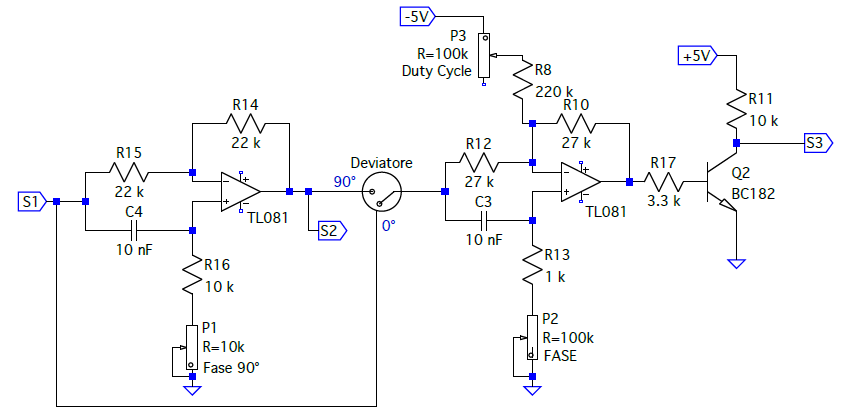
\includegraphics[width=0.5\textwidth]{../grafici/Dephaser.png}
	\caption{Schema del circuito: sfasatore di $90^\circ$ e sfasatore a fase variabile.}
	\label{fig:deph}
\end{figure}

\begin{figure}[H]
	\centering
	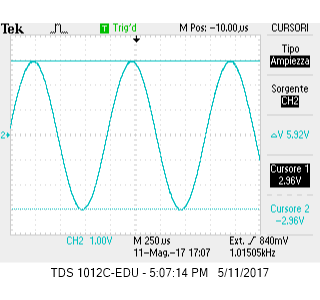
\includegraphics[width=0.5\textwidth]{../grafici/s1.png}
	\caption{Onda sinusoidale inviata in S1.}
	\label{fig:s1}
\end{figure}

\paragraph{Sfasatore di $90^\circ$} 

Lo sfasatore di $90^\circ$ è schematizzato nella prima parte del circuito in \cref{fig:deph} (prima del deviatore). \newline
Modificando la resistenza sull'ingresso non invertente dell'opamp tramite il trimmer $P_1$ si modifica la fase tra l'onda in uscita di esso ($S_2$) e l'onda in ingresso $S_1$. Questo è dovuto principalmente alla presenza del
condensatore $C_4$: se si risolve il circuito, grazie al condensatore $C_4$, si ottiene che l'uscita $S_2$ acquista una componente immaginaria oltre a una reale, ed entrambe dipendono dal trimmer $P_1$. In questo modo cambiando la resistenza all'ingresso non invertente dell'opamp si può fare in modo che $S_2$ sia sfasato di $90^\circ$ rispetto ad $S_1$. Per la precisione ciò che si è ottenuto ruotando $P_1$ è che la differenza di fase in $S_2$ è di $\Delta \phi = 1.53\pm0.04$ rad, da confrontare con il valore nominale pari a $1.57$ rad $(90^\circ)$.

\paragraph{Sfasatore a fase variabile}

La seconda parte del circuito è molto simile alla prima, con l'aggiunta di:
\begin{itemize}

\item un trimmer $P_3$ collegato tra l'alimentazione a -5 V , la terra e, attraverso una resistenza $R_8$, all'ingresso invertente dell'opamp.

\item un transistor Q2 BC182 con l'emettitore a massa, il collettore a +5 V e la base collegata all'uscita dell'opamp.
\end{itemize}

Il trimmer permette di modificare l'offset dell'onda all'ingresso invertente dell'opamp e quindi dell'onda in uscita di esso; in questo modo il transistor, che ha la funzione di interruttore (quindi passa da interdizione e saturazione), cambia il suo stato di "aperto" o "chiuso" per un tempo che dipende direttamente dal trimmer $P_3$. Quindi modificando questo trimmer si agisce direttamente sul duty cicle dell'onda (quadra) in uscita in $S_3$. Si è quindi fatto in modo che quest'onda sia perfettamente simmetrica (duty cycle 50\%), come si può vedere dalla
\cref{fig:3_devposB}.

Come si può vedere dalla \cref{fig:deph} il deviatore permette di decidere se mandare
all'ingresso della seconda parte del circuito l'onda $S_1$ o l'onda $S_2$. 
Si è verificato che agendo sul deviatore si varia la fase di uscita di $S_3$ di
$90^\circ$ rispetto ad $S_1$, come si può osservare confrontando le \cref{fig:3_devposA,fig:3_devposB} con la \cref{fig:s1} (si è verificato esplicitamente tramite l'oscilloscopio che la differenza di fase fosse effettivamente di $90^\circ$, cioè pari a quella ottenuta in $S_2$).

\begin{figure}[H]
\begin{minipage}{0.49\textwidth}
	\centering
	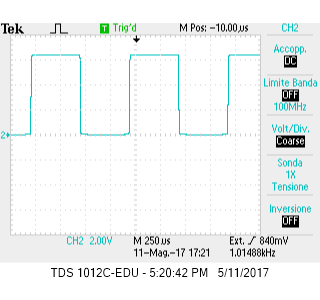
\includegraphics[width=0.8\textwidth]{../grafici/s3_devposA.png}
	\caption{Uscita $S_3$ quando il deviatore è collegato direttamente con $S_1$.}
	\label{fig:3_devposA}
\end{minipage}
\begin{minipage}{0.49\textwidth}
	\centering
	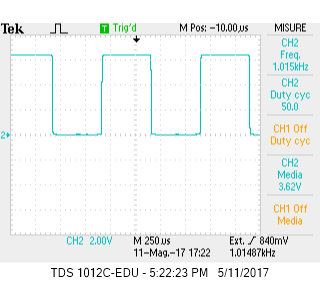
\includegraphics[width=0.8\textwidth]{../grafici/s3_devposB.png}
	\caption{Uscita $S_3$ quando il deviatore è per l'altra posizione del deviatore.}
	\label{fig:3_devposB}
\end{minipage}
\end{figure}

Anche il trimmer $P_2$ modifica lo sfasamento tra l'onda in $S_3$ e $S_1$. Si sono quindi esplorati i limiti sullo sfasamento dettati da questo trimmer, ottenendo che esso può sfasare l'onda di al più $2.70\pm0.08 rad$, cioè di circa $180^\circ$. 



%devo scrivere i valori delle componenti circuitali? io scriverei tutte le specifiche all'inizio nella sezione scopo e strumentazione.

\subsection{Squadratore e campionatore}

\begin{figure}[H]
	\centering
	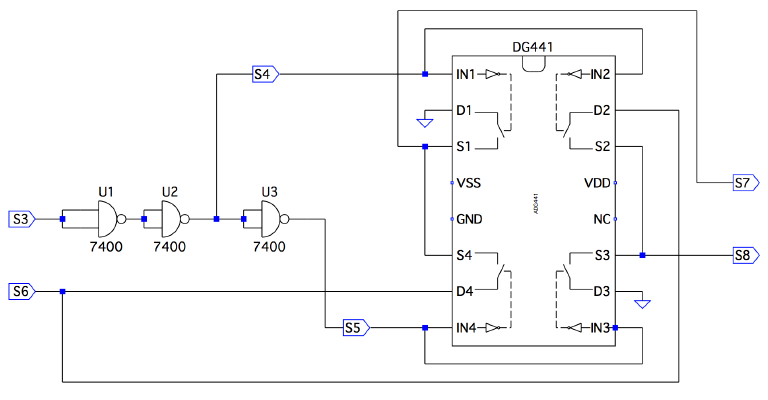
\includegraphics[width=\textwidth]{../grafici/SqSamp.png}
	\caption{Schema del circuito: squadratore e campionatore.}
	\label{fig:sqsamp}
\end{figure}

Il circuito mostrato in \cref{fig:sqsamp} è diviso in due sottocircuiti:
\begin{itemize}
	\item uno identificabile con le tre porte NAND $ U_1, U_2 $ e $ U_3 $;
	\item l'altro costituito dagli interruttori dell'integrato DG$ 441 $.
\end{itemize}

Il primo sottocircuito è molto semplice, e l'effetto delle porte NAND (usate in questo caso come dei NOT) è quello di forzare l'uscita ad assumere come valori i livelli logici \code{HIGH} e \code{LOW} fissati dalle porte.
In questo modo si è ottenuto uno squadratore, la cui uscita è $ S_4 $.

\begin{wrapfigure}{L}{0.5\textwidth}
	\vspace{-10pt}
	\centering
	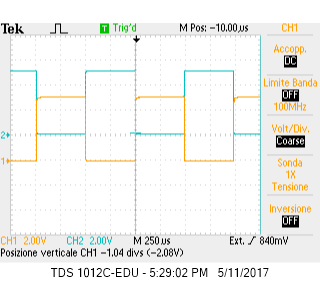
\includegraphics[width=0.4\textwidth]{../grafici/s4s5.png}
	\vspace{-12pt}
	\caption{Uscite $ S_4 $ e $ S_5 $.}
	\label{fig:s4s5}
	\vspace{-12pt}
\end{wrapfigure}

\noindent L'effetto dell'ultimo NAND, $ U_3 $, è quello di ottenere un'altra onda quadra sull'uscita $ S_5 $, in opposizione di fase rispetto a quella su $ S_4 $.

Le due forme d'onda sono mostrate in \cref{fig:s4s5}.
\newline

Il secondo sottocircuito è anch'esso semplice: esso è costituito da quattro interruttori, due dei quali connessi a terra a un'estremità, e gli altri due connessi all'ingresso $ S_6 $.
I quattro interruttori sono controllati in tensione dalle uscite dello squadratore, cioè $ S_4 $ e $ S_5 $, con l'effetto di averne due attivi e due spenti a ogni semiperiodo, e nella configurazione invertita nei semiperiodi adiacenti.
Le estremità libere degli interruttori sono connesse alle uscite $ S_7 $ e $ S_8 $.
\newline

Il risultato ottenuto per queste ultime uscite è mostrato nelle \cref{fig:s7s8,fig:s7s8a90}.

Ciò che accade è che per un semiperiodo una delle due uscite viene connessa a terra, mentre l'altra è connessa direttamente a $ S_6 $, mentre al semiperiodo successivo le onde quadre commutano, e fanno commutare lo stato di tutti gli interruttori, invertendo il ruolo delle due uscite rispetto al semiperiodo precedente.

\begin{figure}[H]
\begin{minipage}{0.49\textwidth}
	\centering
	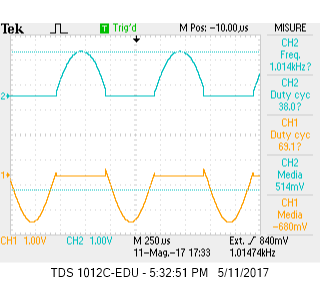
\includegraphics[width=0.8\textwidth]{../grafici/s7s8fasegiusta.png}
	\caption{Uscite $ S_7 $ e $ S_8 $.}
	\label{fig:s7s8}
\end{minipage}
\begin{minipage}{0.49\textwidth}
	\centering
	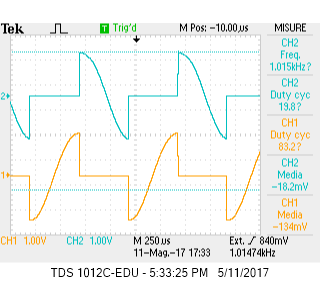
\includegraphics[width=0.8\textwidth]{../grafici/s7s8fasegiusta90gradi.png}
	\caption{Uscite $ S_7 $ e $ S_8 $, altra posizione del deviatore.}
	\label{fig:s7s8a90}
\end{minipage}
\end{figure}

\subsection{Amplificatore differenziale}

\begin{figure}[H]
	\centering
	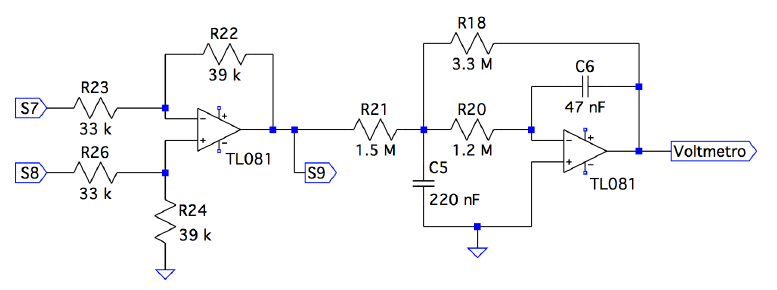
\includegraphics[width=\textwidth]{../grafici/DiffAmpAv.png}
	\caption{Schema del circuito: amplificatore differenziale e mediatore.}
	\label{fig:diffav}
\end{figure}

Se i valori riportati in figura fossero corretti e l'op-amp fosse ideale\footnote{Dunque le tensioni ai capi dei due ingressi fossero perfettamente uguali}, allora l'amplificazione differenziale dovrebbe essere $R_B/R_A$\footnote{Posti $R_B=22, 24$ e $R_A=R23, R26$}

Se si considera che le resistenze non sono perfette (ma si continua a considerare l'op-amp come ideale) l-output dell'amplificatore diventa:

$V_{out}=V_0\frac{R23+R22}{R26+R24}\frac{R24}{R23}-V_1\frac{R22}{R23}$

Per cui l'amplificazione di modo comune e l'amplificazione differenziale valgono rispettivamente:

$A_{cm}=\unit{0.007\pm 0.006}{}$

$A_{diff}=\unit{1.160 \pm 0.014}{}$ 

\subsection{Mediatore}

Il mediatore si può intendere come un unico circuito, oppure come un passa basso messo in serie a un altro circuito. Se si adotta questo schema è però opportuno non trascurare la resistenza di ingresso del secondo circuito, che sebbene sia alta, è comunque comparabile con quella della prima parte del circuito. \footnote{Per C5 e C6 si intende i rispettivi valori dell'impedenza complessa, ovvero $-i/\omega C5$ e $-i/\omega C6$}


$R_{in}=\frac{R18//(R20+C6)}{1-A(\omega)}$

Dove $A(\omega)$ è l'amplificazione della seconda parte del circuito.
L'amplificazione di questa parte è chiaramente non dipende dalla presenza o meno del loop $R18$, che ha il solo scopo di diminuire la resistenza di ingresso del circuito (in \cref{fig:MEDFR} indicata con $Z(\omega)$).

$A(\omega)=-C6/R20$ dunque $R_{in}=\frac{R18//(R20+C6)}{1+C6/R20}=\frac{R18//(R20+C6)}{1+C6/R20}=\frac{R02*R18(R20-\frac{i}{\omega C6})}{(R18+R20-\frac{i}{\omega C6})(R20-\frac{i}{\omega C6})}$

Facendo i conti con la resistenza di ingresso si ottiene dunque...

$V_in'=\frac{C5//R_{in}}{R21+C5//R_{in}}$ e $V_{out}=A(\omega)V_{in}'=-\frac{C6}{R20}\frac{C5//R_{in}}{R21+C5//R_{in}}=-\frac{C6}{R20}\frac{C5//\frac{R18//(R20+C6)}{1+R20/C6}}{R21+C5//\frac{R18//(R20+C6)}{1+R20/C6}}$\\


Dato che questo risultato è abbastanza complicato, si è preferito plottare in \cref{fig:MEDFR} come dovrebbe comportarsi il circuito in frequenza. Questi plot dobrebbero convincere il lettore che l'oggetto si comporta effettivamente come un mediatore sopra frequenze dell'ordine del Hz, mentre lascia passare fluttuazioni a frequenza più bassa (permettendo all'apparecchio di avere prontezza finita).

\begin{figure}[H]
	\centering
	\includegraphics[width=\textwidth]{../grafici/mediatorefr.pdf}
	\caption{Risposta in frequenza del mediatore. Il comportamento dell'op-amp è stato supposto ideale nel fare questi conti.}
	\label{fig:MEDFR}
\end{figure}

Praticamente la resistenza $R18$ ha anche la funzione di impedire il raggiungumento della saturazione del op-amp. Se non ci fosse questa resistenza, infatti, il circuito sarebbe più un integratore ideale che un mediatore, e andrebbe presto in saturazione, rendendo inutilizzabile l'apparecchio.


Si può notare inoltre da \cref{fig:MEDFR} che per $\omega \rightarrow 0$ l'amplificazione tende ad $1$, dunque il circuito tende a fornire una media non distorta del segnale.



\section{Misure di assorbimento}


Sono stati fatti in totale tre misure di assorbimento. I tre test sono stati svolti con tre distanze distanze led-fotodiodo diverse: quelle con distanze minori impediscono di avere un numero cospiquo di lastrine, quelle con distanza maggiore sono più affette a rumore. 


Prima di procedere con le misure sono state fatte delle misure ripetute del valore della tensione con lo switch nell'altra posizione ("zero"). La tensione in questo caso non è zero ma fluttua attorno a quel valore. Si è dunque provveduto a stimare l'errore quadratico medio, che risulta circa di $20 mV$.

Questo si è fatto misurando con i cursori dell'oscilloscopio lo spessore della banda di tensioni, e prendendone il 68\%. %non è vero, ma mi permette di non dover giustificare il non aver stimato l'offset e aver lascito far questo al fit  


Questo si è somato in quadratura al'errore strumentale del multimetro, che è sempre trascurabile. 

Si è dunque fittata la formula $V=V_0e^{-n/b}+c$. Si noti che la costante serve per colpa di un piccolo offset non eliminabile con il multimetro e difficilmente stimabile. L'aggiunta di questo parametro permette di far tornare il test del $\chi^2$. 

Si sono ottenuti i seguenti dati:

\begin{table}[H]
	\centering
	\begin{tabular}{cccc}
		$ N_0 $ & Run 1 [V]& Run 2 [V]& Run 3[V]\\
		\hline
		0 & 1.740+/-0.017 & 2.290+/-0.021 & 1.490+/-0.016\\
		1 & 1.400+/-0.016 & 1.840+/-0.017 & 1.151+/-0.015\\
		2 & 1.180+/-0.015 & 1.500+/-0.016 & 0.930+/-0.015\\
		3 & 0.994+/-0.015 & 1.230+/-0.015 & 0.753+/-0.015\\
		4 & 0.840+/-0.015 & 1.020+/-0.015 & 0.618+/-0.015\\
		5 & 0.715+/-0.015 & 0.810+/-0.015 & 0.510+/-0.014\\
		6 & 0.600+/-0.014 & 0.680+/-0.015 & 0.436+/-0.014\\
		7 & 0.501+/-0.014 & None & 0.358+/-0.014\\
		8 & 0.425+/-0.014 & None & 0.303+/-0.014\\
		9 & None & None & 0.255+/-0.014\\
		10 & None & None & 0.225+/-0.014\\
		11 & None & None & 0.188+/-0.014\\
		12 & None & None & 0.148+/-0.014\\
		13 & None & None & 0.125+/-0.014\\	
	\end{tabular}
\caption{Misure della tensione sull'uscita $ S_6 $ in funzione del numero di piastrine.}
\label{tab:s6}
\end{table}

E sono stati fatti i seguenti fit:

\subsection{Run 1}

$\chi^2/d.o.f.=6.67670880055/6$ \\
$P(\chi^2>\chi^2_{dati})=0.351782036336$\\ 

\begin{figure}[H]
	\centering
	\includegraphics[width=\textwidth]{../grafici/fit1.pdf}
	\caption{Fit del primo run di dati}
	\label{fig:RUN1}
\end{figure}

\begin{table}[H]
	\centering
	\begin{tabular}{cccc}
	Nome	&	$ V_0 $[V] &  b          & a [V]\\
	Valore  & 1.96   & 4.9  & 0.10\\ 
	Errore  & 0.03 & 0.3 & 0.05\\
	\hline
	$V_0$ [V] & 0.00115473  & 0.00675163  & -0.00130441\\
	b  	    & 0.00675163  & 0.0947997   & -0.01453302\\
	a [V]   & -0.00130441 & -0.01453302 & 0.00236345\\
\end{tabular}
\caption{Risultati del fit sul primo set di dati. Sotto la sbarra la matrice di covarianza stimata.}
\label{tab:Run1}
\end{table}

\subsection{Run 2}

$\chi^2/d.o.f.= 2.8/4$ \\
$P(\chi^2>\chi^2_{dati})= 0.59$\\
 
\begin{figure}[H]
	\centering
	\includegraphics[width=\textwidth]{../grafici/fit2.pdf}
	\caption{Fit del secondo run di dati}
	\label{fig:RUN2}
\end{figure} 

\begin{table}[H]
	\centering
	\begin{tabular}{cccc}
	Nome	&	$ V_0 $[V] &  b      & a [V]\\
	Valore  &   2.73 & 4.58  & 0.08\\
	Errore	& 0.04   & 0.25  & 0.06\\ 
\hline 
	$V_0$ & 0.00198996 & 0.00880121  &-0.00255638\\
 	b     & 0.00880121 & 0.06458724  &-0.01631311\\
 	a     &-0.00255638 & -0.01631311 & 0.00428632\\
\end{tabular}
\caption{Risultati del fit sul secondo set di dati. Sotto la sbarra la matrice di covarianza stimata.}
\label{tab:Run2}
\end{table}

\subsection{Run 3}

$\chi^2/d.o.f.= 13.7/11$ \\
$P(\chi^2>\chi^2_{dati})= 0.25$\\

\begin{figure}[H]
	\centering
	\includegraphics[width=\textwidth]{../grafici/fit3.pdf}
	\caption{Fit del terzo run di dati}
	\label{fig:RUN3}
\end{figure} 



\begin{table}[H]
	\centering
	\begin{tabular}{cccc}
	Nome	&	$ V_0 $[V] &  b      & a [V]\\
	Valore  &  1.75  & 4.26 & 0.081\\
	Errore	& 0.02 & 0.14 & 0.014\\ 
\hline 
	$V_0$ & 4.80334423e-04 & -1.29715106e-03  & 1.92105673e-05\\
 	b     & -1.29715106e-03 &  1.99359641e-02 & -1.78714278e-03\\
 	a     &  1.92105673e-05 & -1.78714278e-03 &  2.02730982e-04\\
\end{tabular}
\caption{Risultati del fit sul terzo set di dati. Sotto la sbarra la matrice di covarianza stimata.}
\label{tab:Run3}
\end{table}

\subsection{Conclusioni}

Si riportano dunque i valori così ottenuti:

\begin{table}[H]
	\centering
	\begin{tabular}{cccc}
    - & Run 1 & Run 2 & Run 3\\
Valore & 4.9 & 4.58 & 4.26\\
Errore & 0.3& 0.25 & 0.14\\
$P(\chi^2)$ & 0.35 & 0.59 & 0.25\\
\end{tabular}
\caption{Risultati}
\label{tab:Results}
\end{table}

Si nota che sebbene i risultati del test del $\chi^2$ siano positivi, i valori ottenuti dalle tre misure non sono in accordo alla interno degli errori sperimentali. Si presume dunque che gli errori siano stati sovrastimati e il test passi sebbene non il modello non sia perfettamente attinente ai dati. 

La non correttezza del modello può essere dovuta a diversi fattori. Si può ad esempio pensare a una possibile non linearità del fotodiodo rispetto alla luce assorbita. 

Di fatto la noncorrettezza del modello può essere anche notata dalla visibile forma ottenuta in tutti e tre i grafici degli scarti normalizzati, che è frotemente correlata fra i diversi esperimenti indipendenti, dunque non può essere una fluttuazione non sistematica.

Di fatto la migliore sitma del coefficente di attenuazione è:

$b_{best}=4.43 \pm 0.11$ lastre.%Mo' mediare i risultati non ha senso...quindi non lo faccio...dovrei infatti pesare la cosa con il x^2...alla fine l'ho fatto lo stesso...
A questo risultato è meglio abbinare anche la semidispersione (stima dell'errore massimo, e utile in quanto il modello non riproduce perfettamente i dati), $\Delta b=0.32$ lastre. 

\end{document}